\chapter{Introduction}
\label{chapter1}

Robots are emerging from controlled factories and
laboratories into our homes, workplaces, roads, and public airspaces.
Alongside their transition into these unstructured and transient environments
comes their need to be able to explore, characterize, and catalog their surroundings.
Mobile robot autonomy is generally accomplished by referring to a map - a 2D or 3D
probabilistic representation of the locations of obstacles in the robot's workspace.
With access to a map, robots can localize to determine their position, plan collision-free
trajectories to goals, locate objects for interaction, and make decisions by
reasoning about the geometry and dynamics of the world. Given that a robot's map
is of critical importance for most autonomy tasks, robots that find
themselves initialized without a priori access to a map should be capable of
autonomously, efficiently, and intelligently creating one.

The exercise of choosing and executing actions that lead a robot to learn more about its own
map is known as \textit{active perception} or \textit{exploration}, and
is the central topic of this thesis. Active perception has previously been studied with a
multitude of sensor models, environment representations, and robot dynamics
models. The active perception task itself can be dissected into two
components~\cite{shen20113d}:

\begin{enumerate}[leftmargin=3.2cm]
  \item[\bf component 1:] Identifying regions in the environment that, when visited, will
    spatially extend or reduce uncertainty in the current map
  \item[\bf component 2:] Autonomously navigating to the aforementioned regions, while
    simultaneously localizing to the map and updating it with acquired sensor
    measurements
\end{enumerate}

\begin{figure}[ht]
  \centering
  \includegraphics[width=0.6\textwidth]{example-image.png}
  \caption{A household service robot awakes in an unknown environment. Prior to
  accomplishing its main functionalities, it will require a map of its surroundings.
What sequence of actions should it take to minimize the time it spends
exploring? \label{fig:motivation}}
\end{figure}

A motivating example is depicted in Fig.~\ref{fig:motivation}, where a household
service robot is initialized in an unknown environment. Prior to accomplishing
tasks that a human might ask it to perform, the robot must learn its
surroundings and build a map of the house. Ideally this phase of
initialization would be fast, as it is a prerequisite to the main functionality
of the robot, and also might be required when furniture is moved or
household objects are displaced. Where should the robot travel to observe the
most of the environment in the shortest amount of time? Virtually any autonomous robot
operating in an unknown environment will require a map-building
initialization phase, welcoming strategies that enable high-speed and intelligent
exploration.

This thesis introduces an assortment of information-theoretic optimizations that
increase the efficiency of active perception when using a beam-based sensor
model (e.g. LIDAR, time-of-flight cameras, structured light sensors) and
an occupancy grid map~\cite{elfes1989using}. Applying these optimizations during exploration allows a
robot to consider a significantly larger number of future locations to move
towards in its partially observed environment, regardless of the planning
strategy used. Additionally, this thesis presents a method for analyzing the
complexity of the local environment and adapting the robot's map resolution,
planning frequency, movement speed, and exploration behaviors accordingly. By
adapting these properties online, an autonomously exploring robot is able to speed up
through areas with open expanses or where the map is well-known, and slow down
when the local environment requires careful maneuvering or more thorough
investigation.

\section{Previous Work}

Prior approaches to mobile robot active perception fall into two
broad categories: \textit{geometric} approaches that reason about the locations and
presence of obstacles and free space in the robot's
map~\cite{acar2002sensor,chan1993line,wang2007view,
burgard2000collaborative,taylor1993exploration,yamauchi1997frontier}, and more
recently, \textit{information-theoretic} approaches that treat the map as
a multivariate random variable and choose actions that will maximally reduce its
uncertainty~\cite{amigoni2010information,bourgault2002information,charrow2015icra,
julian2013mutual,feder1999adaptive}. Both categories of approaches solve {\bf
component 1} of active perception, and assume that a planner and Simultaneous
Localization and Mapping (SLAM) framework are available to accomplish {\bf
component 2}.

\subsection{Geometric Exploration Strategies}

Many successful geometric exploration approaches build upon the seminal work of
Yamauchi~\cite{yamauchi1997frontier}, guiding the robot to \textit{frontiers} - regions on the boundary
between free and unexplored space in the map (Fig.~\ref{fig:frontiers}).
Since multiple frontiers often exist simultaneously in a partially explored map, a
variety of heuristics and spatial metrics can be used to decide which frontier to
travel towards~\cite{lavalle2006planning}. For example, an agent may decide to
visit the frontier whose path through the configuration space from the agent's current
position has minimum length, or requires minimal time or energy input to
traverse. Similarly, an agent may decide to only plan paths to locations
from which frontiers can be observed by its onboard sensors.

\begin{figure}[hb]
  \centering
  \includegraphics[trim=0cm 0.4cm 0.1cm 0.1cm, clip, width=0.8\textwidth]{frontiers.pdf}
  \caption{A partially explored map with frontiers between free and unknown
  space highlighted in blue.\label{fig:frontiers}}
\end{figure}

While effective in 2D environments, frontier exploration algorithms have
several restrictive qualities. First, the na\"{i}ve extension of frontier exploration
from 2D to 3D maps poses a non-trivial challenge; as the
dimensionality of the workspace increases, frontiers are distributed more
densely throughout the environment due to occlusions, sensing resolution, and
field-of-view, resulting in poor exploration performance~\cite{shen20113d}.
Second, planning a path to a frontier does not imply that the path
itself will be information-rich. Trajectory optimization techniques that
consider information acquired by the robot's sensors along a planned path can be used
as extensions to improve exploration performance~\cite{sim2004online,kollar2008trajectory}.
Finally, although the robot is guaranteed to learn new information upon reaching a
frontier, the amount of information learned is dependent on the
robot's sensor model, which is not considered when identifying frontiers.
It may therefore be more efficient to visit a frontier that is
suboptimal according to heuristics such as path length if the robot's sensors
will provide more information from that location
(Fig.~\ref{fig:sensor_frontier}).
This limitation was first overcome by evaluating the informativeness of simulated
sensor measurements taken from frontier locations~\cite{gonzalez2002navigation}, and was the
original motivation for developing a category of information-theoretic exploration strategies.

\begin{figure}
  \centering
  \centering
  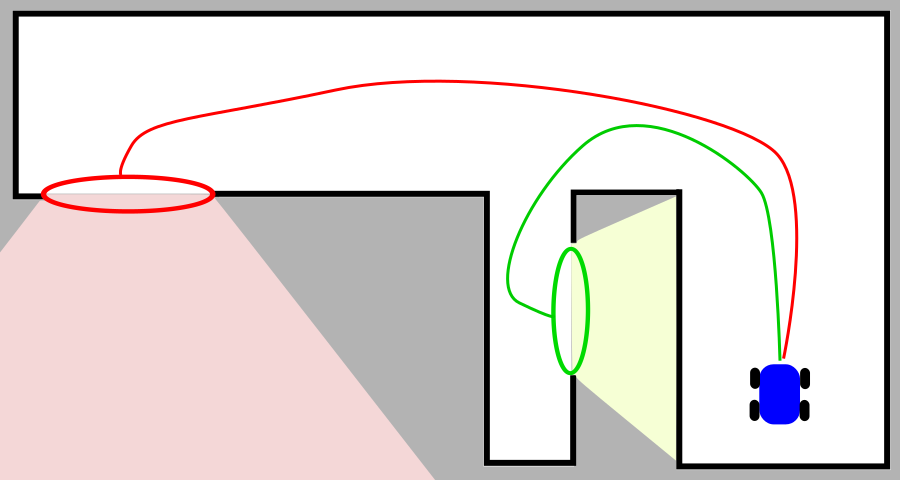
\includegraphics[width=0.7\textwidth]{sensor_frontier.pdf}
  \caption{Traditional frontier exploration would visit the green location first
    because it is closest. A simple extension involves simulating sensor
    measurements from frontiers and examining their informativeness~\cite{gonzalez2002navigation}. Applying this
    extension would cause robot to visit the red frontier first, since that
    location will provide more information about the map per unit time.\label{fig:sensor_frontier}}
\end{figure}

More thorough surveys of frontier exploration algorithms and heuristics are provided by
Basilico et al.~\cite{basilico2008evaluating} and Holz et al.~\cite{holz2011comparative}.

\subsection{Information-Theoretic Exploration Strategies}

Information-theoretic exploration strategies cast the active perception task as
an optimization, and choose actions for the robot that maximize an information-based objective function such
as Shannon's entropy or mutual
information~\cite{bourgault2002information,kollar2008efficient,charrow2015icra,julian2013mutual}
(Fig.~\ref{fig:mi_vs_csqmi}).
Entropic measures like these are appealing because unlike geometric methods,
they capture the relationship between sensor placement and uncertainty in the
map. In addition, they can be computed without a maximum likelihood map estimate, and
therefore do not discard probabilistic information known to the robot. Control policies
that maximize mutual information have been proven to guide robots
towards unexplored space~\cite{julian2013mutual}, and weighting frontiers by
the expected mutual information between the map and a sensor measurement
acquired at the frontier location has been shown to result in more efficient exploration
behaviors than traditional frontier exploration~\cite{charrow2015icra}.
The exact same calculation can be used to evaluate information-theoretic objective
functions in 2D and 3D environments.

\begin{figure}[b]
    \centering
    \begin{subfigure}[t]{0.31\textwidth}
        \centering
        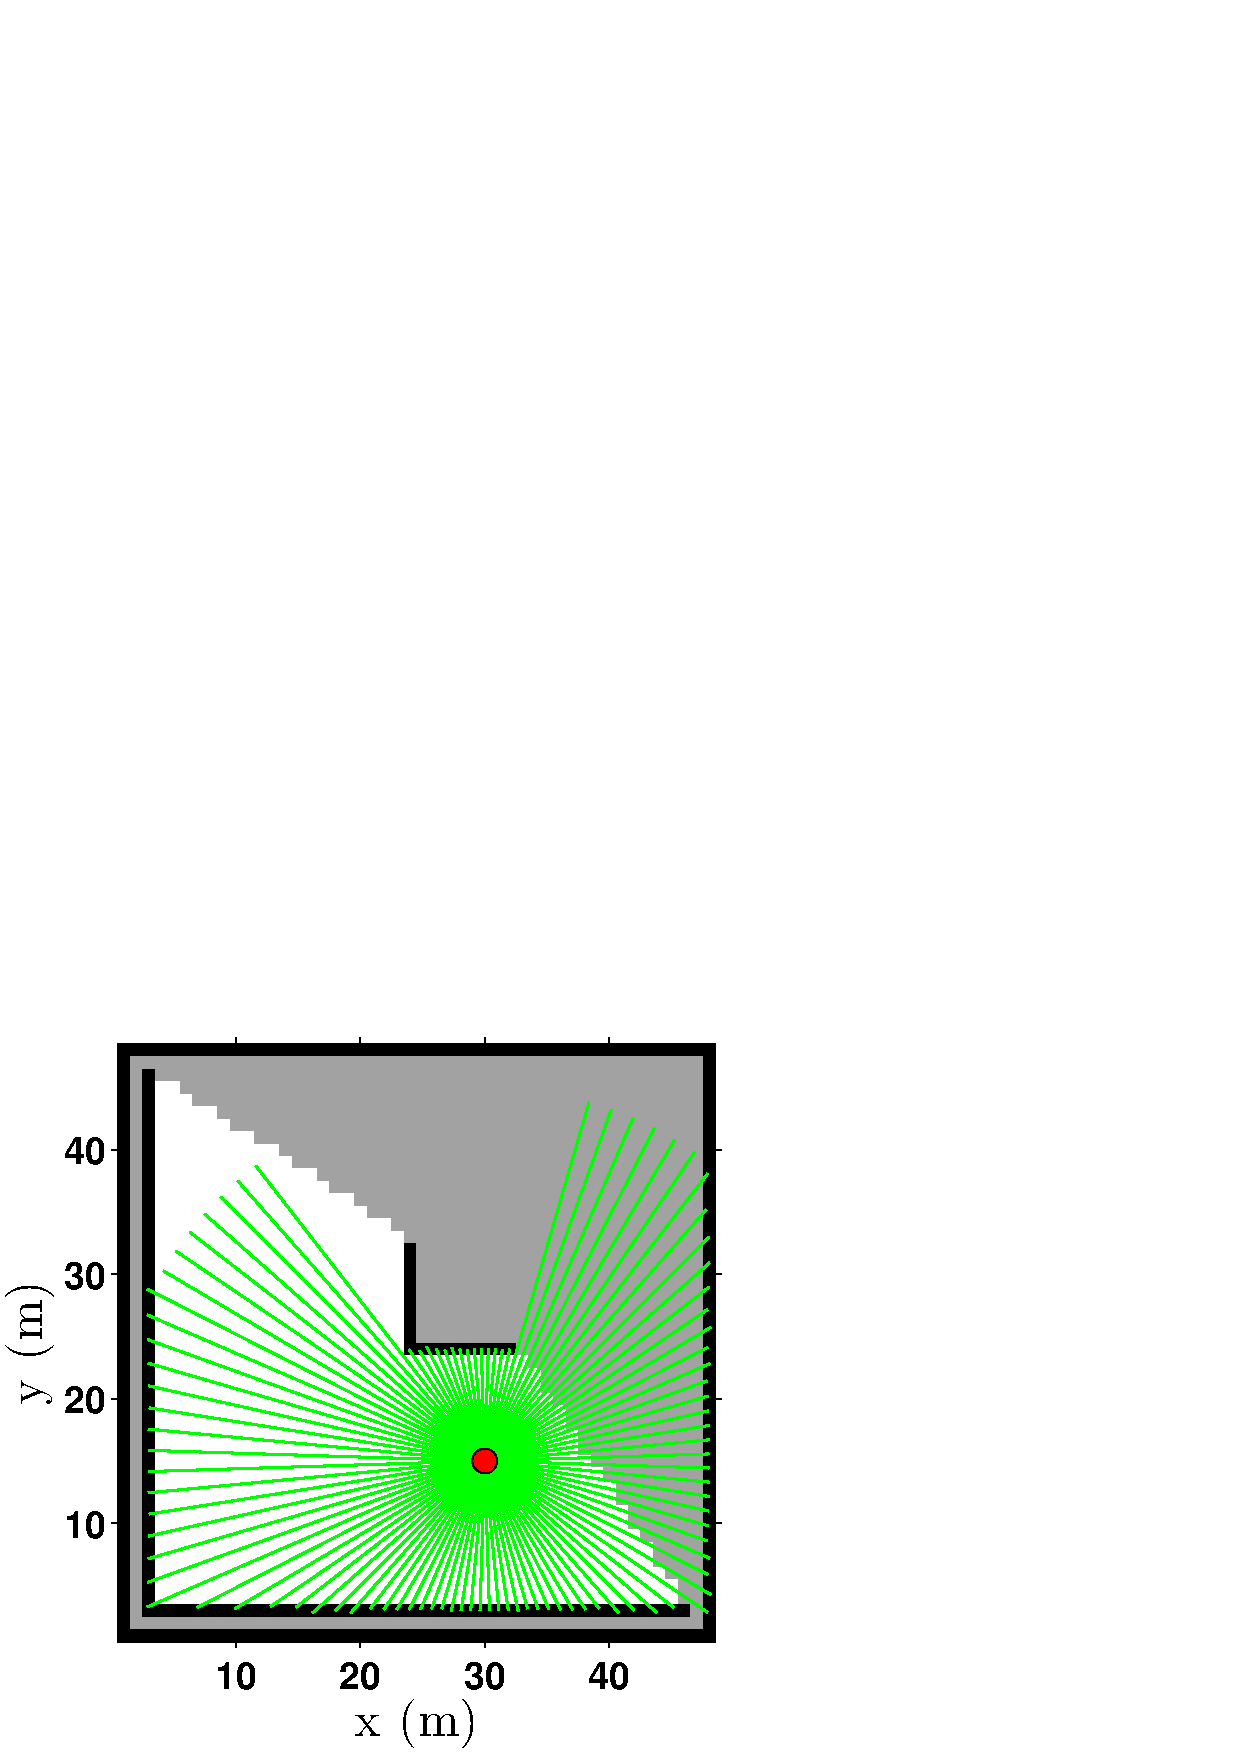
\includegraphics[height=4.0cm]{map.pdf}
        \caption{\label{fig:og}}
    \end{subfigure}
    \begin{subfigure}[t]{0.31\textwidth}
        \centering
        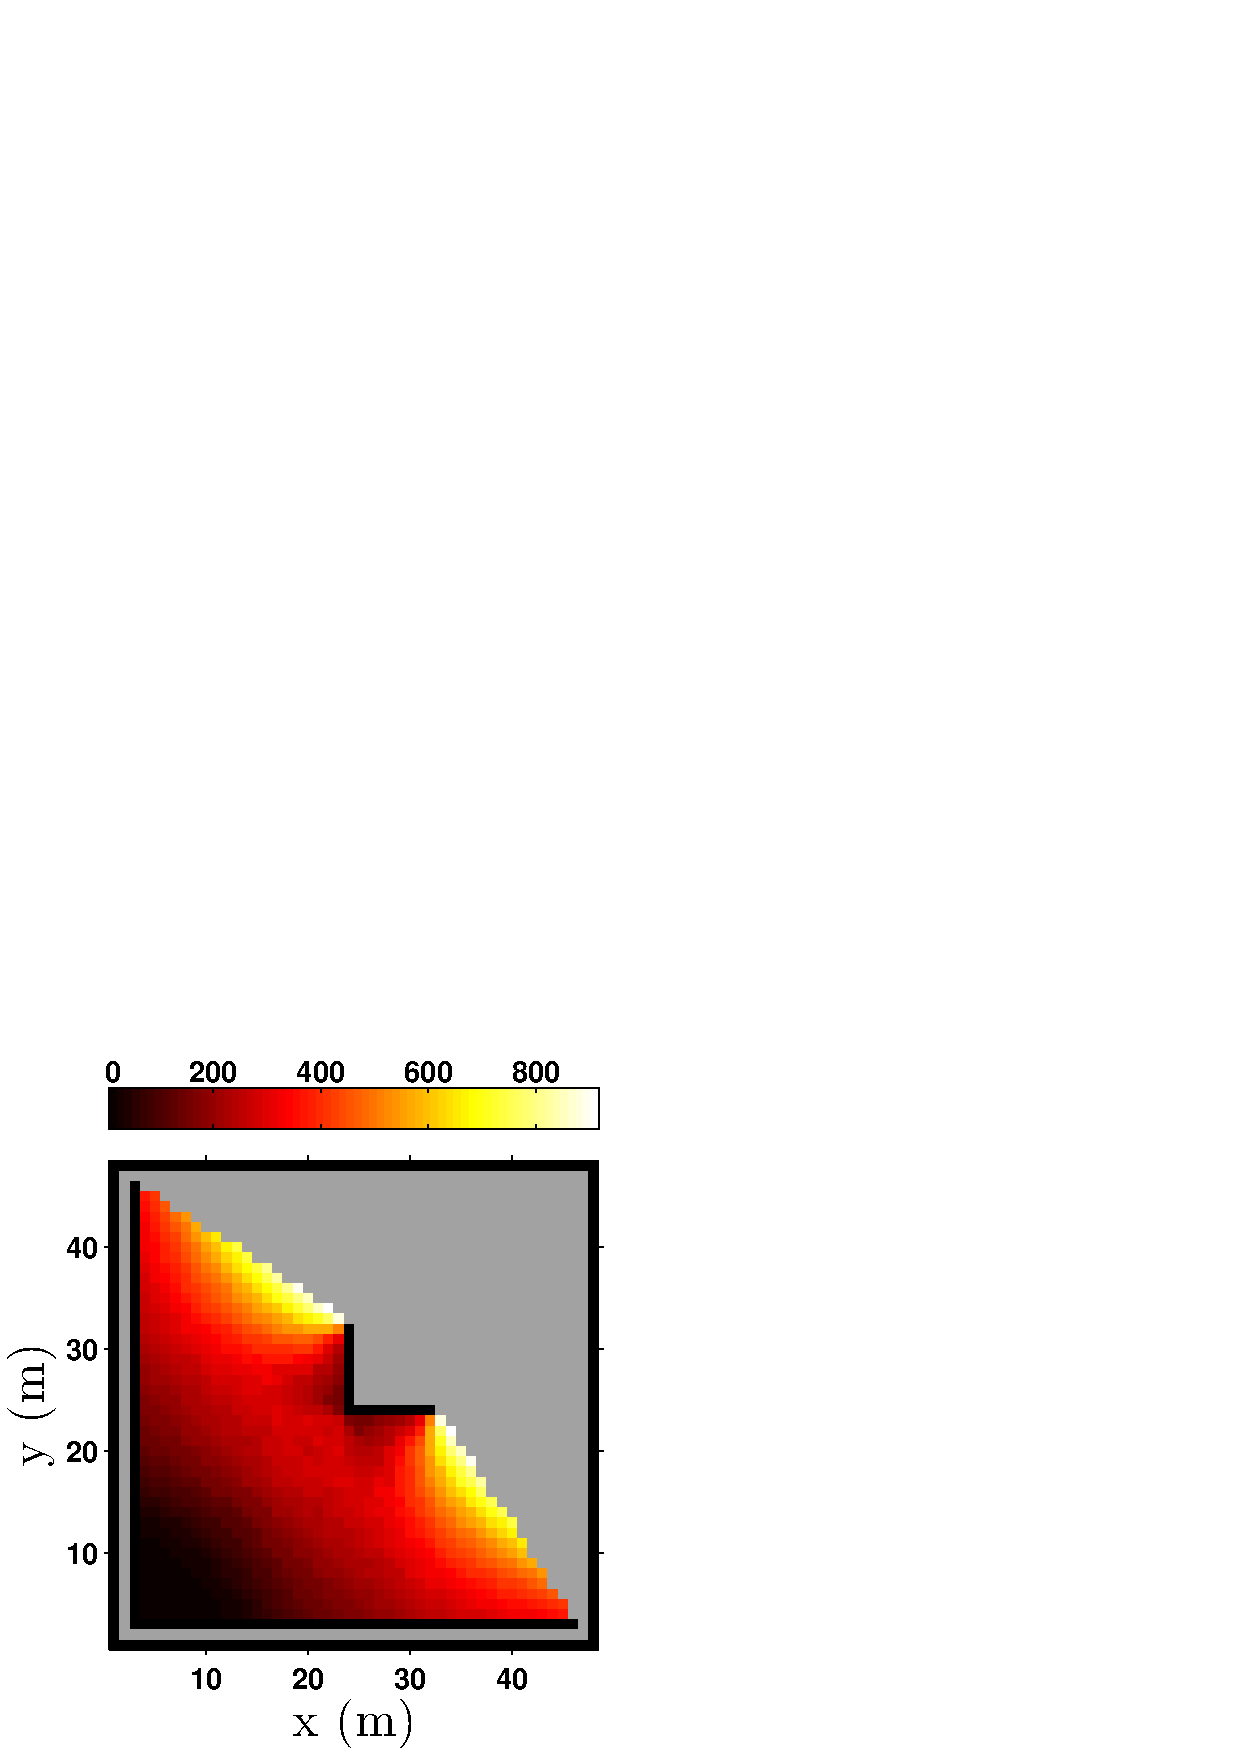
\includegraphics[height=5.0cm]{mi_map.pdf}
        \caption{\label{fig:og_mi}}
    \end{subfigure}
    \begin{subfigure}[t]{0.31\textwidth}
        \centering
        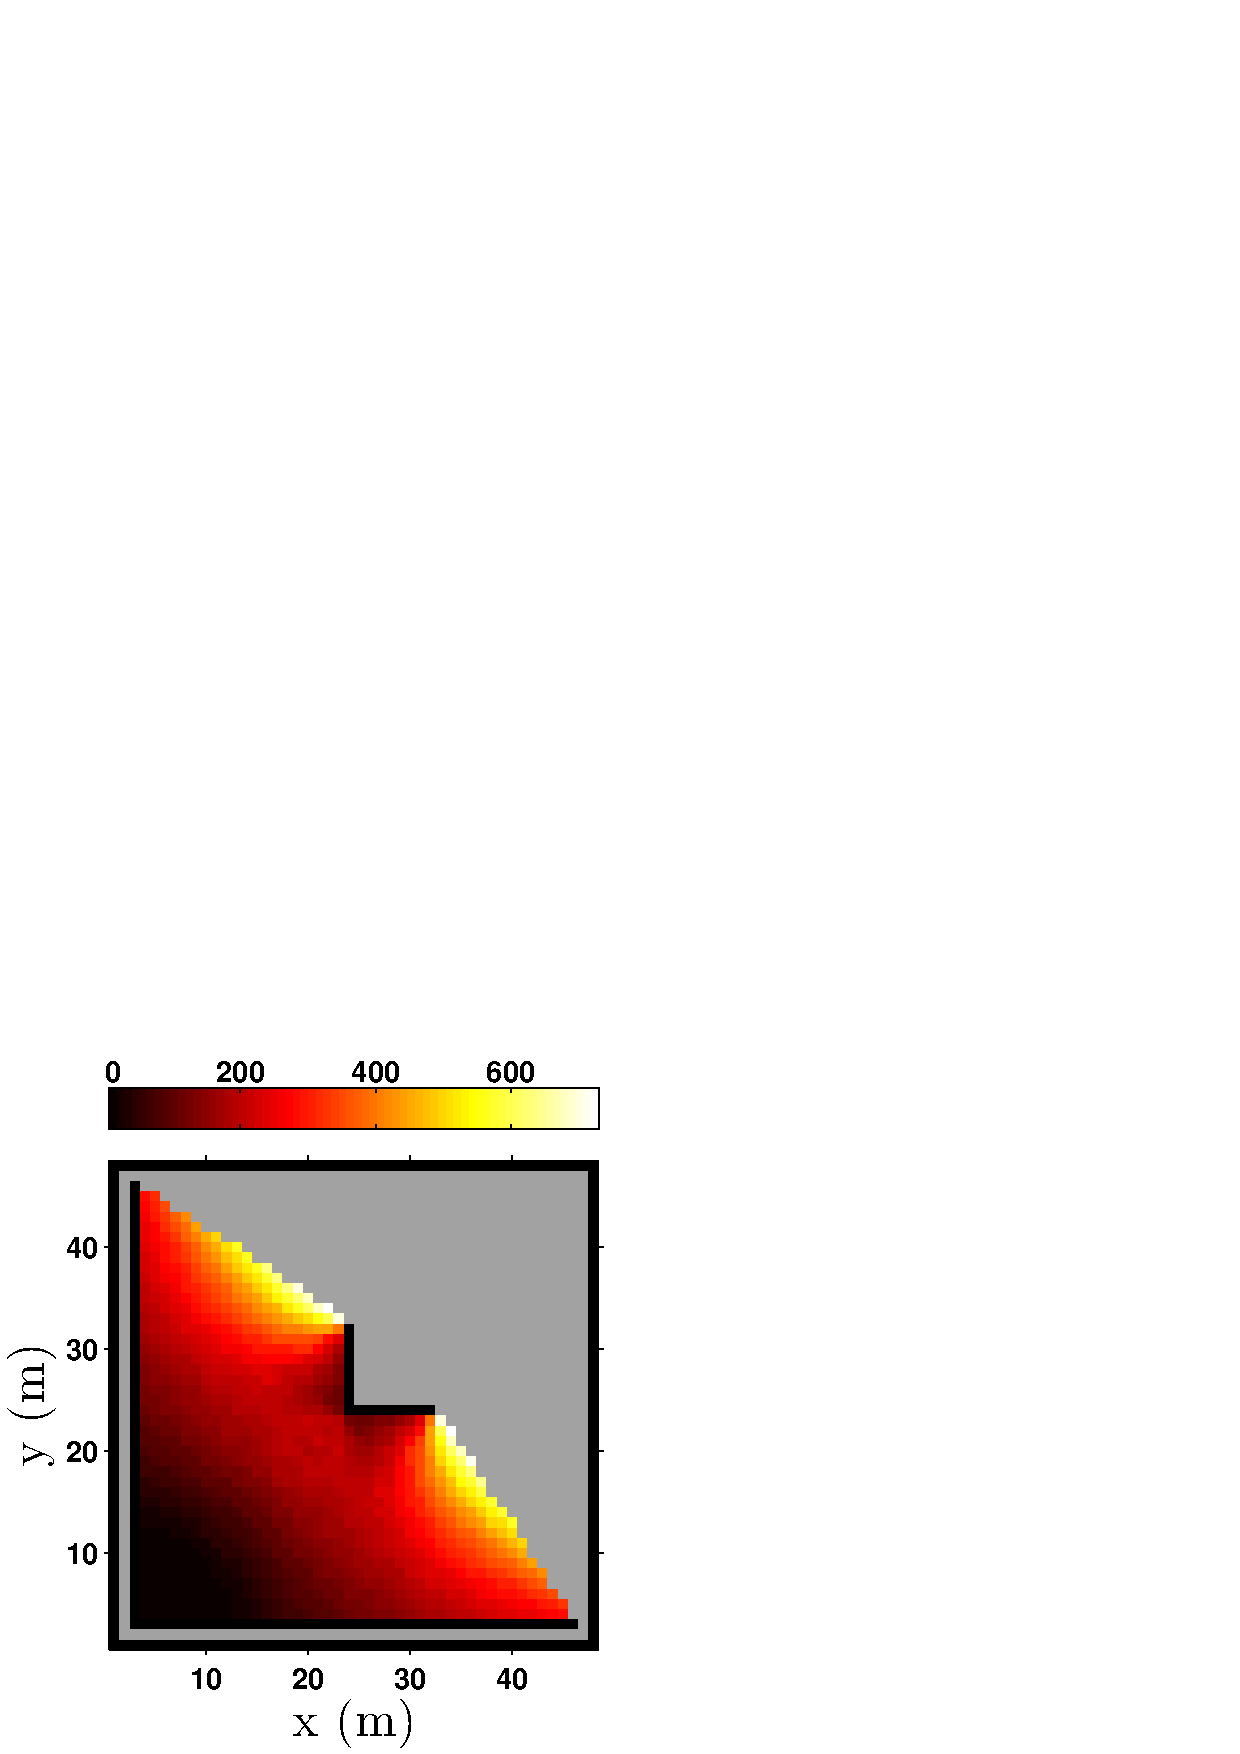
\includegraphics[height=5.0cm]{csqmi_map.pdf}
        \caption{\label{fig:og_csqmi}}
    \end{subfigure}
    \caption{Two variants of mutual information (Fig.~\ref{fig:og_mi}: Shannon;
    Fig.~\ref{fig:og_csqmi}: Cauchy-Schwarz Quadratic) densely computed in free space
  over an occupancy grid (Fig.~\ref{fig:og}) using a $100$-beam omnidirectional 2D
laser with $30$ m range. An exemplary sensor measurement is depicted in
Fig.~\ref{fig:og}. Controlling the robot towards locations that maximize either variant
of mutual information would attract the robot to locations from which it
could observe unknown areas of the map. \label{fig:mi_vs_csqmi}}
\end{figure}

The utility afforded by information-theoretic approaches comes at the cost of
computational inefficiency.
As a point of comparison, frontiers and other geometrically-defined landmarks
need only to be computed once per map update, and can be computed (at worst, using a brute force search)
with time complexity linear in the number of cells in the robot's map.
One may alternatively choose to identify and cache frontiers every time a sensor
measurement is used to update the map, yielding a constant time frontier
identification step that is bounded by the number of map voxels within the maximum sensor range.
By contrast, information-theoretic objective functions typically consider the probabilistic
uncertainty associated with the sensor and environment models, and therefore
require expensive sensor-related operations such as raycasts or sampling a large
number of times from the distribution of possible future measurements.
Approximations to mutual information between a map and beam-based sensor
measurements can be evaluated with time complexity linear in the number of map
voxels intersected by a sensor's
beams~\cite{julian2013mutualthesis,charrow2015icra,nelson2015iros}. This
already-expensive operation must be performed for every future location that the
robot might wish to travel to. Julian et al. report that densely calculating
mutual information over the free space in a large $1500$ m$^{2}$ map requires
approximately ten seconds with a parallelized implementation using a $3.4$ Ghz
quad-core CPU and NVIDIA GTX 690 graphics card~\cite{julian2013mutual}.

\section{Thesis Problem}

Although inefficient, information-theoretic solutions to the active perception task
are superior to geometric solutions in many ways. However, modern computers cannot densely
evaluate information-theoretic objective functions over a robot's map in real-time.
Any strategy that makes the evaluation of information-theoretic objective functions more
efficient will allow a robot to consider more future locations prior to taking
an action towards one, thereby increasing the speed at which the robot is able
to explore an environment.

Currently, the most efficient information-theoretic exploration algorithms are
too slow for the motivating scenario described in
Fig.~\ref{fig:motivation}. For example, a highly-efficient recent approach
by Charrow et al., requires eleven minutes to explore a $17$ m $\times 18$ m $
\times 3$ m building with a quadrotor - enough time for the quadrotor's batteries to
deplete twice~\cite{charrow2015icra}. This thesis addresses the inefficiencies of information-theoretic exploration,
summarized in the following statement:

% Thesis Problem
\begin{center} \fbox{
  \parbox{0.9\linewidth}
  { {\bf Thesis Problem:} Solutions to the mobile robot active perception task
  that involve optimization of information-theoretic cost functions are too
  computationally expensive for high-speed exploration in complex environments.}
} \end{center}

\section{Thesis Statement}

This thesis proposes occupancy grid compression as a solution to
the computational inefficiencies of information-theoretic exploration.

\section{Outline}




